\begin{figure*}
\centering
    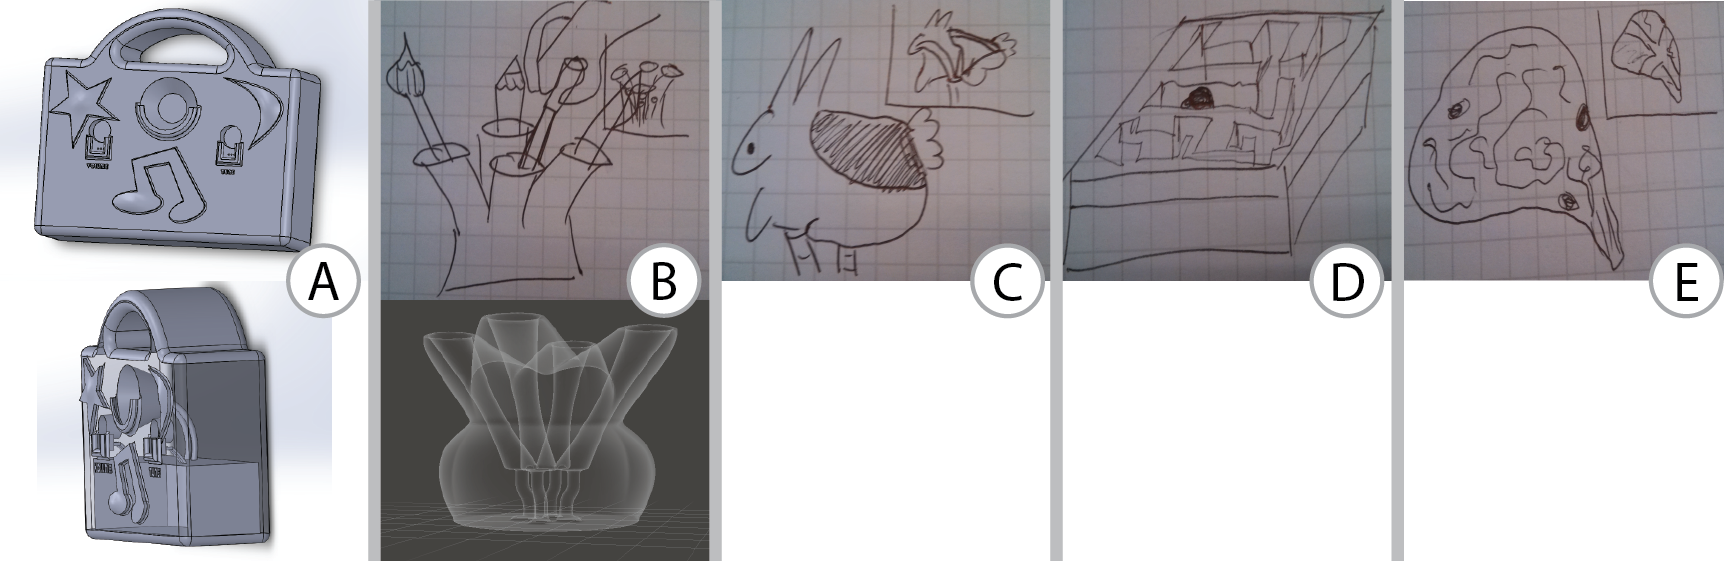
\includegraphics[width=7in]{figures/examples.png}
\caption{A series of example objects created using our system.  (a) is a touch-sensitive brain toy.  (b) is a rabbit which ``breathes'' using wind pipes we built.  (c) shows a portable radio.  (d) shows a presence-aware pen holder.  (e) is a maze game.}
\label{fig:examples}
\end{figure*}

\section{Example Objects}

To evaluate and highlight our tool's capabilities, we fabricated a set of five prototype objects designed using a Series of Tubes.  All prototypes were fabricated in a single piece, unless described otherwise.

\subsection{Touch-sensitive Toys (open, liquid, star, terminals)}

In order to demonstrate our star topology feature and show how conductive fluids can be used for touch sensing, we created a set of touch-sensitive toys and a companion app, reminiscent of the boat application in Acoustic Barcodes \cite{Harrison-acoustic}. The objects --- a brain and boat, in our example --- can be set on a base, which announces ``brain'' or ``boat'', and also the names of special features on the object when they are touched. For example, touching the brain model's front protrusion yields the announcement ``olfactory bulb''. The distinct touch points on each object are connected by an interior star topology of tubes filled with conductive copper paint, and touch sensing is performed via a single wire and SFCS (see Figure \ref{fig:toys}).  We built a smart base which can distinguish between the toys and also determine which toy is mounted: since each toy and each gesture has a distinct capacitive signature, we use a simple classifier trained to detect both toy and gesture based on profile.

The models we used for the toys' exteriors were all downloaded from the free website Thingiverse.  All components were fabricated on a Makerbot, support-free.  After printing, we injected copper paint (CuPro-Cote) into the interior pipes using a craft syringe.  This paint requires approximately 2 days to fully dry in this configuration (3mm diameter tubes, maximum tube length 10cm).  Our smart base is powered by an Arduino Uno running open-source SFCS code\footnote{http://www.instructables.com/id/Touche-for-Arduino-Advanced-touch-sensing/?ALLSTEPS}.

\subsection{Breathing Bunny (semi-closed, gas, terminals)}

To demonstrate how gases can be used to both provide sensation to the user through openings and to deform a model internally, we created a rabbit with a pair of tubes that can simulate breathing (see Figure \ref{fig:breathe}).  When the rabbit inhales through its nose, its abdomen rises, and as it exhales its abdomen falls.  For this, we used a combination air/vacuum pump: one terminal creates a vacuum while the other creates positive pressure.  Our rabbit has two pipes, one open tube exiting at its mouth and one semi-closed pipe capped with rubberlike material in its abdomen.  We connected one pipe to each of our pump's terminals, and using a programmable power supply we mimic a rabbit's breathing pattern.  This example was printed on our Objet in rubberlike material, with support flushed post-print.

\subsection{Custom Radio (open, threadable, terminals)}

A custom radio, built using pipes integrated with traditional electronics, allows users to tune to different stations and listen in.  This device uses a network of disconnected open pipes threaded with wires to connect our components (two potentiometers, an LED, and a speaker) to a microcontroller (Arduino Pro Micro). We hid the microcontroller and a battery-driven power supply in the base of the radio to make it portable.  For the radio functionality, we attached an Si4703 radio tuner breakout board to the Arduino, which offers headphone-jack output.

In order to create so many pipes (3 per potentiometer, 1 for the LED, 1 for the speaker) and still preserve surface quality after voxelizing, we added a "High Quality" for pipe-cutting.  This mode voxelizes at a resolution of 512x512x512 instead of our previous 128x128x128.  It does preserve surface geometry, however it requires around 3 minutes to complete a single cut operation, compared to our nearly-instant smaller voxel grid (computation on a 3D grid increases by the cube of the 1D size increase).  We fabricated the radio itself on our Makerbot, support-free but cut in two pieces to allow the Arduino and battery pack to be inserted.

\subsection{Presence-aware Pen Holder (open, solid, ternimals)}

Our presence-aware pen holder can distinguish which tool or tools a user has picked up (see Figure \ref{fig:pens}).  Our pen holder uses a modification of the FlyEye technique described by Wimmer in \cite{Wimmer-flyeye} and contains open tubes filled with fiber optic cables, one per pen chamber.  We use a single cable per chamber; our 6mm diameter fiber optic cables, in comparison to the fine tubes used in the original work , can send and receive through the same cable.  At the base of each tube is a QRE1113 line sensor digital breakout board, which has an integrated IR emitter and receiver.   When a pen is in its appointed place, the emitted infrared light is reflected off its bottom and travels back to the receiver, where it registers as bright.  This prototype was built by our Objet and support was flushed post-print. \valkyrie{this whole paragraph is unclear}

\subsection{Animated Neon Sign (return, threadable, path)}

\begin{figure}[h!]
\centering
    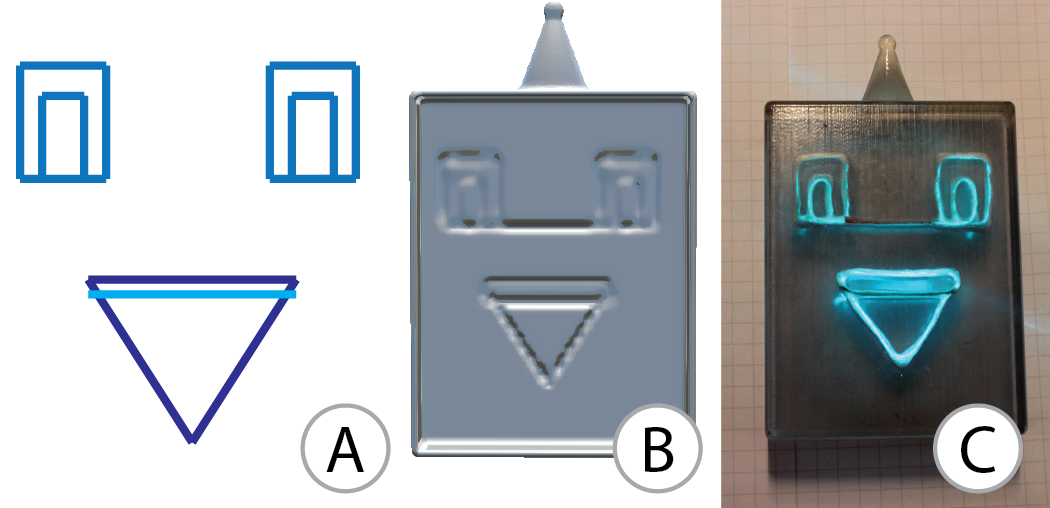
\includegraphics[width=3.4in]{figures/sign.png}
\caption{A two-state animated neon sign designed using our tool.  (a) shows the input SVG files, with the two states of the mouth drawn in different colors. \bjoern{it's hard to tell these apart!}  (b) shows the resultant mesh when we subtracted the generated tubes. \bjoern{hard to see what's going on here, too.} In (c), we show the fabricated sign.}
\label{fig:neon}
\end{figure}

Neon art, perhaps best known for its association with Las Vegas, is traditionally made from hand-formed glass tubes containing neon gas.  The tubes light up when a current is passed through them.  For this type of art, the path of the tubes is of crucial importance, as it determines how the sign will look.  We designed a custom neon robot head which can be animated to ``talk''.  The pipes have been threaded with EL wire which is lit in sequence to create an animation.  Our sign was fabricated on the Objet in two halves, cutting through the plane of the sign itself, and with pipes cut in the rear piece to allow the wire to exit backwards and hide the EL wire controls.  The EL wire was threaded post-print, and is controlled by an EL wire sequencer.

\subsection{Maze (fully enclosed, particulate, tree, terminals + path)}

Using a modification of our graph-based algorithm which only cuts the literal drawing (and does not perform Eulerization, etc.), we created a maze game with a single particle trapped in a fully enclosed tube.  This maze is based on an SVG we created by hand and processed with our internal path tube tool.  To fabricate the tube, we created it in two halves that were fastened together via glue, due to limitations in our ability to remove support material otherwise. \bjoern{observant reviewers will call us out on this - that many of our techniques may not actually be workable in a single piece because you can't get the support material out. I think if you had a lye bath you could actually get more complicated models done, as long as you're patient and there's some entry and exit for the lye to reach all pipes.}  \valkyrie{we should discuss.  I will try to get a model of this ready ASAP}  We created this prototype on our Objet in two halves, inserting a marble before closing.